\documentclass{article}
\usepackage{graphicx}
\usepackage{amsmath}
\graphicspath{ {files/RCP_diagram/} {files/}}

\title{Multi-Scale Resolution of Human Social Systems:  A Synergistic Paradigm for Simulating Minds and Society}
\author{Mark G. Orr}

\begin{document}
\maketitle

\section{Introduction}
Recently, we put forth an initial sketch of what we call the \textit{Resolution Thesis}\cite{orr2018brims}.  The thesis holds that 1) models of cognition will be improved given constraints from the structure and dynamics of the social systems in which they are embedded, and 2) the resolution of social simulations of agents will be improved given constraints from cognitive first principles\footnote{Cognition considered as theoretical models of human perception, thought and action that includes, broadly, explanations of emotion, motivation, and affect in addition to more tradtional domains of cognitive psychology and cognitive science; one could arguably use the term \textit{psychological first principles} as equivalent.}.  This thesis reflects a variety of motivations, the most obvious being the observation that there is little overlap between the cognitive sciences and the generative social science approach, both of which rely heavily on computer simulation to understand aspects of human systems, albeit at different levels of scale.  The former focuses almost exclusively on the mind as a scientific object of study for which the lion's share of simulation efforts reflect methods that represent a generalizable conception of the mind and the latter emphasizes multiple aspects of social systems, the mind being only one of these aspects. Thus we have a trade-off: the details of one level of scale result in the potential oversimplification at the other level of scale.  We posit, by the resolution thesis, that an interdependence between cognitive science and generative social science could be leveraged for the purposes of improving our understanding of important phenomena studied by both.    

The \textit{Resolution Thesis} can be understood from multiple perspectives.  From the generative social science perspective, the \textit{Resolution Thesis} means that the representations of agents in social simulations should be informed closely by cognitive science and relevant neurophysiological considerations.  This runs somewhat counter to the principled adherence to simplification of the internal processing of simulated agents found in this literature, a simplification that served to show that complex social dynamics can be driven by simple behavioral rules of agents.  

More recently, there have been efforts in the generative social sciences that acknowledged that closer ties to the psychological and neurophysiological underpinnings of human behavior may yield benefit in terms of modeling social phenomena.  Epstein's neurocognitive approach is a notable effort in this vein\cite{epstein2014}; there are other related approaches (e.g. \cite{caillou2017,sakellariou2008,malleson2012}).  However, there still remains a large gap between these recent efforts and the implementation of models from cognitive science and psychology, not necessarily in principle, but in practice. It is worth noting that there are some threads in cognitive science that approach social modeling from the perspective of cognitive science.  In particular, Ron Sun's push for multi-agent systems based on cognitive first principles is notable\cite{sun2006}; other work in this vein exists\cite{Bhattacharyya2010,lebiere2000,reitter2012,romero2014,gonzalez2003,fu2007,huberman1998,west2001,west2005}.  The relatively new field of computational social psychology is clearly relevant\cite{vallacher2017} as well as the computational organizational theory approach\cite{prietula1998}.

From the view of cognitive science, the \textit{Resolution Thesis} means that patterns of organization (e.g., information flow on the internet, clustering of behaviors in a community) at the social and organizational level should inform cognitive models when appropriate\footnote{The appropriateness may not be easily determined; for social cognition it may be obvious, but it may not be as clear for other domains, e.g., visual categorization.}.  In other words, these patterns should be included as convergent evidence for a theory or model of cognition.  At first consideration this notion may seem hard to fathom because the implications of cognition for the structure and dynamics of social systems are little understood from the cognitive science perspective\footnote{Anderson's Relevance Thesis\cite{anderson2002}, a somewhat rare exception, reasons about how cognition may have implications for social organization.}.  Without an explanatory scheme that links facets of the cognitive model to aspects of social organization, how do we interpret the convergent evidence from social systems?  The work mentioned above with respect to the cognitive first principles within the generative social science approach \cite{sun2006,Bhattacharyya2010,lebiere2000,reitter2012,romero2014,gonzalez2003,fu2007,huberman1998,west2001,west2005} begins to put in  place a better understanding of the implications of cognition on social systems, but does not generally consider simulation output as part of the convergent evidence for theory at the cognitive level of scale.  This is a subtle but critical point, so let us put it differently.  From the congitive perspective, simulation of social systems with agents grouded deeply in cognitive first principles does not imply the \textit{Resolution Thesis} unless the simulation results are used to judge the quality of the cognitive first principles that ground the agents.  

A third and more general view is that the \textit{Resolution Thesis} is about human social systems.  An understanding of any of these levels of scale is dependent, to some degree, on an understanding of the others.  In effect, the notion of convergent evidence as originating, in part, from other levels of scale, applies to all levels of scale.  The implication is that we should leverage information across scale in an iterative and synergistic way. 

The \textit{Resolution Thesis}, despite sounding somewhat reasonable at face value, is opposed, to some degree, from both the cognitive science and generative social science perspectives.  Simon's notion of nearly decomposable systems--that the temporal dynamics of adjacent levels of scale, in most systems, are little correlated--suggests that we can understand well the dynamics at each level of scale independently of the others\cite{simon1962}(see \cite{anderson1972}, for similar arguments in physical systems).  The KISS principle (keep it simple, stupid) used heavily in the generative social sciences, is clearly akin to Simon's notion, and is bolstered by its early wins in understanding the behavior of social systems using simple, non-cognitive agents\cite{schelling1969,axelrod1995,epstein2002}.  In cognitive science, Newell, in considering the time scale of human behavior, suggested that the social band ($> 10^4$ seconds, representing social systems and organizational behavior) is characterized to be weak in strength in the sense that it may not reflect computations in a systematic purposeful way relative to lower temporal bands, e.g., cognitive and neural processes\cite{newell1990}.  

These counter arguments notwithstanding, our working assumption is that the degree to which the  \textit{Resolution Thesis} is useful is an empirical issue.  The state of the art in technology and computing and the tight coupling between them and the current social mileau should afford exploration of the Resolution Thesis.   To this end, we've developed the \textit{Reciprocal Constraints Paradigm} (henceforth \textit{RCP}), a methodological approach for exploring the  \textit{Resolution Thesis}. The value of the \textit{RCP} does not lie in precise formal prescriptions, but in providing a scaffold for growing our understanding of social systems, and, possibly revealing something new about the interdependencies among levels of scale.  

\section{The Reciprocal Constraints Paradigm}
Figure \ref{fig:rcpdiagram} shows the four primary components of the \textit{RCP}: a cognitive system with potential ties to neurophysiology, a social system, and the constraints between levels of scale.  We assume that social systems and cognitive systems are derived from and exhibit an abstract set of first principles \& properties, called $S$ and $C$, respectively (e.g., theoretial entities, experimental paradigms, patterns in empirical data in respect to the discipines that address a particular level of scale).  Defining $S$ and $C$ will depend on the social system or cognitive system of interest.  The notion of constraint simply refers to the use of information from $S$ \& $C$ to inform one another in a principled way. An upward-constraint refers to information from the cognitive level as informing the social level of scale; downward-constraints reverse this relation.


\begin{figure}
	\centering
	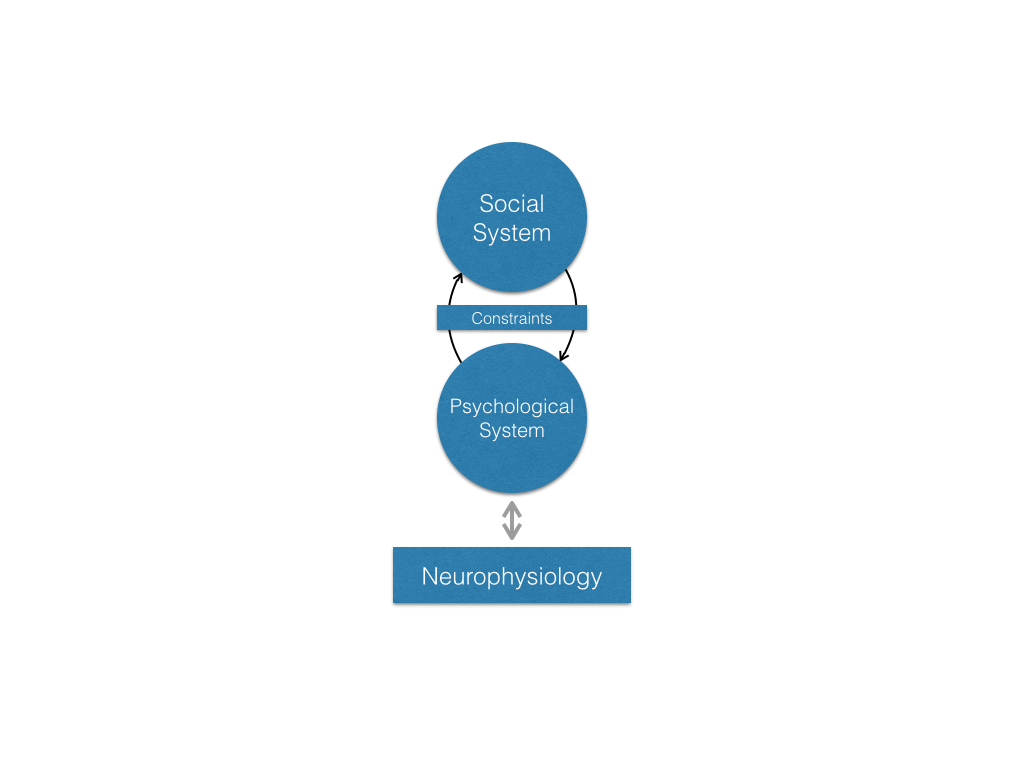
\includegraphics[width=1.0\textwidth]{RCP_diagram.png}
	\caption{\label{fig:rcpdiagram} The four components of the \textit{RCP} are a cognitive system with potential ties to neurophysiology, a social system, and the constraints on each one from the other.  In the \textit{RCP} social systems and cognitive systems are assumed to be derived from and exhibit an abstract set of first principles \& properties, called $S$ and $C$, respectively.  Also captured here is the potential for integrating neurophysiolgical considerations into the cognitive system when appropriate; these may prove as essential for some social systems (the grey two-headed arrow indicates this potential). The notion of constraint refers to the use of information from $S$ \& $C$ to inform one another in a principled way.  
	}
\end{figure}



A primary example of entities from the cognitive level of scale are the set of allowable algorithms $A$ such that $a \in C$. That is, $A$ defines algorithms that are grounded in and thus recognized by work in cognitive science and psychology.  Primary examples at the social level of scale are the social structures, channels of information, and dynamic aggregate signals of behavior (e.g., a distribution of degree in a social network over time) that characterize a social system, a large fraction of which are formalized using graph theory/network science.    It is important to emphasize that within $S$ are notions regarding the behavior of agents, not only social structures.

A central assumption in the \textit{RCP} is that cognitive systems and definitions of agent behaviors in social systems are meant to represent human information-processing capacities that can be described as mathematical functions\cite{van2008tractable} \footnote{This is equivalent to Marr's computational level\cite{Marr1982}.}. Thus, at the cognitive level of scale $C$ we can define a cognitive system as $\psi_{ct}: I_{ct} \rightarrow \psi_{ct}(i)$ where $I_{ct}$ is the set of allowable inputs and $\psi_{ct}(i)$ is the output; in $S$ we have a corresponding agent definition as $\phi_{at}: I_{at} \rightarrow \phi_{at}(i)$ where $I_{at}$ is the set of allowable inputs and $\phi_{at}(i)$ is the output for an agent\footnote{Social and cognitive systems may define parameters regarding variability among a set of agents; this is not reflected here.}. 

\subsection{Applying the Reciprocal Constraints Paradigm}   
In practice there are multiple approaches available for application of the \textit{RCP}, but what unites them is the study of a human social phenomena, either defined at one level of scale or at multiple levels of scale.  Naturally, the first step is to identify a social phenomena of interest, a task that is inherently tied to one's perspective.  If the perspective is largely cognitive, then the focus would most likely be on understanding the psychological processes, representations, etc. in relation to social systems, but informed in some way by entities at the social level of scale $S$.   Another perspective, at the social scale, would dictate a concern with the social structures and dynamics of the social system (multiple humans interacting) with some degree of constraint from cognitive first principles.  These two perspectives are both what we call single-scale approaches to the \textit{RCP}. Of course, one could take a multi-scale perspective that draws from both and likely depends on a simulation approach that captures aspects of $C$ and $S$ in one runnable system.  

We will address the obvious issues and difficulties in applying the \textit{RCP} after providing a description of some potential methods for application.  The goal in this section is simply to express what it might look like to apply the \textit{RCP}.  

\subsubsection{Single-Scale Approaches}
The single-scale approach of the \textit{RCP} aims to elucidate or refine a model at one level of scale by using some information from another level.  

Consider the cognitive scale. The single-scale approach amounts to mapping some properties of social systems to properties of cognitive systems for the purpose of identifying potential implications of social structure and dynamics that should be considered when evaluating a model of cognitive process or representation.  For example, suppose one has in hand a cognitive model of how humans acquire attitudes from social interactions (via some learning process) that has not yet been evaluated against empirical data.  From the perspective of the \textit{RCP}, proper evaluation of the model (of attitude acquisition) would incorporate or consider aspects of the social level of scale that may have implications for the cognitive system.  

In this hypothetical example, we might start with the observation that cognitive learning mechanisms are known to be sensitive to the sequential order in which information is presented to the system \footnote{We see this phenomena broadly, for example,  in attitude formation\cite{cacioppo1992rudimentary}, categorization\cite{heit1994models}, and text comprehension \cite{mcnamara1996learning}.}.   Also, we might observe that, at the social level of scale, the patterning and dynamics of social interactions are dependent upon some properties of $S$ if $S$ contains graph $G$ where $V(G)$ and $E(G)$ are the agents and information channels, respectively. Thus, graph $G$ may have implications for the hypothesized inputs to the attitude acquisition model in terms of the distribution and sequential ordering of features that the attitude model cares about (e.g., beliefs).  

What do these observations in aggregate (one at each level of scale)  tell us about how to evaluate the cognitive model of attitudes?  The notion, from the perspective of the \textit{RCP} is that some consideration for how networks affect the distribution of and sequential ordering of the inputs should be incorporated into the design of the empirical observations.  Generating random distributions of inputs might not suffice because the hypothesized cognitive model may be representing something in humans that is sensitive to networked information flow.  In short, understanding the flow of information on networks might increase the realism of the experimental context used to evaluate the cognitive model. 

This is one example of trying to understand the implications of social properties on cognitive systems; what this means precisely would depend on the social phenomena of interest (e.g., early language development may depend on a different $G \in S$ compared to racial stereotypes or large-scale population biases in attitudes).  

At the social level of scale there is a similar approach--mapping the properties of cognitive systems to social systems to reveal potential implications from the former to the latter.  An obvious approach is an analysis of the degree to which the definitions of agent behavior $\phi_{at}$ compares to any cognitive system $\psi_{ct} \in C$ for the purpose of clarifying to what degree a social agent seems to be aligned with cognitive first principles.  For the case in which the agent behavior definitions and the cognitive system $\phi_{at}$ and $\psi_{ct}$ are formally well defined, this might be relatively straightforward\footnote{Potential methods for such a comparison would, ideally, focus not only on the comparison of input/output functions but also the nature of the runnable algorithms.}, but this is in no way guaranteed. 

Certainly, there will be cases for which $\psi_{ct}$ is not formally defined\footnote{Many theoretical entities in psychology are not formalized in precise mathematical or computational terms but in terms of experimental methods and the relative interpretation of results using statistical methods and reasoning.}.  In fact, a likely scenario is that the closest matching cognitive system $\psi_{ct}$ for the phenomena at hand is only defined in terms of an experimental paradigm, somewhat ill-defined, non-formal theoretical entities and an interpretation of empirical data resulting from application of the experimental paradigm that respects the theoretical entities.  So, in this scenario, how does one go about comparing an existing definition of agent behaviors $\phi_{at}$ defined in a social system to the properties of a cognitive system $\psi_{ct}$ when the nature of the two representations are vastly different?  This is not a trivial task, but one approach would be to exploit the experimental paradigm that is used to define the cognitive system $\psi_{ct}$ in a manner that affords exploring the definitions of agent behavior as defined by $\phi_{at}$.  In other words, one could mimic the existing experimental paradigm that is the basis for the cognitive system through simulation with agents standing-in for humans (assuming $\phi_{at}$ is defined algorithmically).  In essence, this is like running a psychological experiment on artificial agents, an approach that is already common in computational psychology and cognitive science.  The output of the simulations could be compared to the patterning and dynamics of human performance in the original  empirical data on humans.  This is one suggestion of many potentials, but we hope it illustrates well the potential difficulties.  
  
In summary, although the single-scale approach does not represent the full-blown resolution thesis, it might afford better resolution of a target level of scale by considering some of the implications of other levels of scale. The specific phenomena of interest will drive the precise approaches used.

\subsubsection{Multi-Scale Approaches}
The multi-scale approach is simple in principle: build a simulation platform that simultaneosly captures essential aspects of both the social and cognitive systems $S$ and $C$ in respect to a social phenomena of interest (e.g., an agent-based model of cognitive agents).  The upward-constraints would mean defining agent definitions $\phi_{at}$ from cognitive first principles. The downward-constraints, generated by some measure of how well the simulation social system matches the empirical regularities as defined by the phenomena of interest, would serve as a signal that would suggest modifications to $S$, $C$ or both.  If this scheme seems simplistic, the details of its application are not. 
 
We will illustrate using a hypothetical example. Imagine we're interested in the patterning of obesity by race/ethnicity, a phenomena of interest with key social and policy aspects (e.g., cultural attractor states, social and shared-enviromental influence, spatial patterning co-occuring with racial segregation and residential mobility) and, in fact, a pre-existing set of social simulations from which to draw (see \cite{nianogo2015agent}).  Assume we adopt one of the existing simulation approaches, none of which incorporate much in terms of cognitive first principles in $C$.  Given this starting point, one approach would be to substitute a suitable cognitive system $\psi_{ct}$ for the agent behavior definitions $\phi_{at}$  while keeping the other aspects identical to the original simulation. In other words, we would infuse cognition into the agents.  

To do this, because the context is within a simulation environment, there is a minimum requirement that the inputs to and outputs from the cognitive system $\psi_{ct}$ match what the simulation environment has available (for input) and expects as output relative to agents.  However, a deeper concern is to find a substitution that is theoretically reasonable (similar to the arguments made above with respect to the single-scale approach to social systems) from a potentially limited but variable set of candidate $\psi_{ct}$ to consider, some or none of which might closely resemble the agent behavior definitions $\phi_{at}$. For this hypothetical example, we could draw from several candidates in the health behavior tradition, each of which might be considered as different (e.g., \{$\psi_{ct_i}, \psi_{ct_j}, \psi_{ct_k},...,\psi_{ct_n}$\}).  Choosing among such alternatives may be difficult or may limit the degree to which aspects of the agent behavior defined by $\phi_{at}$ that can be captured by substitution.

We are now, already, at an interesting point in this hypothetical scenario because it yields potentially difficult decision points.  For example,  if $\phi_{at}$ does not match any existing $\psi_{ct_i}$, what is implied?  We might assume that the agent behavior definitions $\phi_{at}$ might not align with what we know about obesity behavior at the cognitive level of scale.  Or, it could be argued that the health behavior field, in respect to the processes for which the agent model was developed to study, has yet to develop a cognitive system $\psi_{ct_i}$ that matches $\phi_{at}$.  One could easily complicate this decision point further or add layers of complication, but we wanted to point out that it gets complicated, fast, with non-trivial solutions, e.g., the development of a cognitive model of a specific health behavior that is grounded empirically takes substantial effort and resources.  

However, let us assume that we find a suitable existing cognitive system $\psi_{ct}$ to substitute for the agent behavior definitions $\phi_{at}$. Our next task would be to consider the downward-constraints.  Imagine that along with a pre-existing social simulation from which to co-opt, come empirical data, judged of adequate quality, that could be used to compute an objective function with respect to the simulations accuracy given our substitution of $\psi_{ct}$ for $\phi_{at}$. This signal, then, would serve as the downward-constraint; i.e., a signal that may indicate issues with the cognitive model\footnote{One might reasonable use the difference between accuracy given $\psi$ and $\phi$ instead for comparison purposes.}.  

Let us assume that the simulation does poorly in terms of accuracy; what is to be done?  One might conduct a set of Monte-Carlo simulations to measure the departure from accuracy with respect to the parameters of the cognitive system $\psi_{ct}$ and consider optimizing these parameters to maximize accuracy. But, this raises a subtle concern--some would argue that not all parameters in $\psi_{ct}$ should be free to vary on theoretical grounds\cite{reitter2010}.  So, we could take this concern into account for our optimization approach.  

It would be reasonable at this point, especially given the potential insights that the Monte-Carlo simulations might provide, to revisit the cognitive model and consider it from multiple angles.  What is the empirical basis of the model?  It is replicated?  What was its purpose originally?  Has the model been used across several applied settings?  Are the assumed cognitive processes and representations grounded in other similar models of similar phenomena?  Given a deep dive into the cognitive model, there might be several options for improving the simulation.  Would this spur further experimentation at the cognitive level of scale? What would this look like?  Would a new experimental paradigm be generated that respected the structure in the agent-based model?  These are all possibilities.

Another concern, aside from issues with the cognitive model, is that unless the properties in $S$ captured in the simulation completely reproduce the empirical data (within a reasonable degree of tolerance), one needs to consider, given the objective function, whether to vary some components in the simulation that represent something in the social system $S$ instead of or in addition to features of the cognitive system $C$. 
  
The above scenario is but one approach, one that is largely \textit{fixing the social system $S$ and importing a cognitive system $C$}.  But what if we \textit{fix $C$ and generate $S$} instead?  What does this look like?  We will stay with the obesity example from above, but change the scenario such that we don't know about any simulation approaches that represent mainly $S$.  Instead, imagine that what we know about the social system $S$ is a set of population-level empirical studies, some of which include information on social networks and the built environment, and some theoretical statements about peer-influence on social networks. Furthermore, similar to the scenario above, there is a limited set of candidate cognitive systems to consider (\{$\psi_{ct_i}, \psi_{ct_j}, \psi_{ct_k},...,\psi_{ct_n}$\}) in the health behavior tradition and, likely, other relevant aspects of the cognitive system $C$ may not be represented in them (e.g., categorization, learning, and memory processes).  Further, only one of these candidate $\psi_{ct_i}$ is in a computational formalism\footnote{There do exist a small handful of computationally implemented health behavior theories; see \cite{orr2017readbook} for a review.}.  We decide that $\psi_{ct_i}$ will serve as our starting point and call it simply $\psi_{ct}$.  

Analysis of $\psi_{ct}$ reveals that it captures the learning and on-the-fly formation of attitudes towards specific health behaviors (considered a precursor to behavior); it is composed in a general manner such that it applies to virtually any health behavior, and; it is empirically grounded using traditional health behavior theory measurment techniques (in one particular behavioral domain). 

These features are useful, but some key components are missing that are akin to first principles of social system $S$.  In particular, $\psi_{ct}$ is mute with respect to the generation of social structure and related dynamics (e.g., decision making for initiating/dissolving relationships; social influence mechanisms in terms of how others' behavior or attitudes can potentially serve as the input to the cognitive system $\psi_{ct}$).  Thus, at minimum, some decision points arise in terms of how the simulation implements generation and change in network structure the mechanism of social influence.  

To this end, one could start by implementing a static network topology that captures regularities found in empirical studies of human social networks and disallow change in the network ties as the simulation progresses.  In terms of social influence, we might assume that what is spreading are attitudes and that exposure to others' attitudes can serve as input to an agent\footnote{We've implemented prototypes of this sort\cite{orr2017galeabook}.} and, further there is a knowable stochastic function between attitude and behaviors relating to obesity, e.g., energy balance behaviors relating to caloric intake and use). At this point, we could build out further the social structure and dynamics in relation to the problem of interest using both theoretic and empirical components from $S$, e.g. racial/ethnic distributions in obesity.  

Notice, that what is going on here is a process of building from a cognitive kernel and adding layers of assumptions from $S$ where $S$ includes different kinds of information\footnote{This is very similar to standard practice in social simulation that uses agent-based approaches except that the kernel starts from first principles of computational social psychology.}  At some point, we need to run the simulation and determine how to apply the downward-constraint. We explore this next.

Once the simulation is runnable, the downward-constraint could operate, as describe above, by computing an objective function with respect to the accuracy of the simulation compared to extant empirical data at the social level of scale.  Here, the issues are mainly the same as in the \textit{fixing $S$ and importing $C$} case described above.

%In this case, although, depending on the provenance of the data sources (to mean, roughly, which level of scale do they originate from), there will be decision points in terms of whether to modify $C$ or $S$, 

%the focus should, at least initially, be on $C$.  

%There is an interesting specific case when fixing $C$ and generating $S$  

%In the limiting case, imagine that the only data we have is from $C$, e.g., some behavioral studies that reveal something about the learning and formation of attitudes about obesity related behaviors and the relation between attitudes and the behaviors.  All of these studies, further, were conducted at the individual-level and reveal little about social structure and dynamics.  In this case, the objective function would be computed with respect to how well $\psi_{ct_i}$ captures the variation in these data alone.  In this case, it is possible that aspect of both $C$ and $S$ could be modified in the simulation to optimize the objective function.  What is interesting about this limiting case is that $C$ may still depend on $S$.  Getting the $S$ right would be essential in a real-world empirical causal sense.

These two examples are largely hypothetical versions of the multi-scale approach to the \textit{RCP}.  The value, we hope, is to provide some sketches of what it might look like in practice.  Clearly, there are many issues that are raised, even by these sketches, let alone by the general notion of the \textit{RCP} and the \textit{Resolution Thesis}. 

%\section{An Example of RCT Implemented}
%We now offer an examle of a multi-scale approach to the \textit{RCP}.  It is a highly stylized example that focues much on $C$ using the cognitive architecture ACT-R with some properties of a specific social domain, online social coding in GitHub.  In particular, [describe simulation sketch here]. 

%It will be useful to introduce ACT-R before continuing to the simulations.  ACT-R is a specific approach to modeling human cognition that invokes the idea of a cognitive architecture, a computational instantiation of the structures, mechanisms and represenations of the mind that are coherent with respect to another notion, that of a unified theory of cogntion\cite{newell1990}. A cognitive model that is developed using a cognitive architecture has a potential a constrains operations (if you will it constraints $\psi_{ct}$ to limits of the human mind w.r.t. a unified theory of cognition standpoint.  Cognitive models based on architectures are structured algorithms of $\psi_{ct}$, and, thus, not strictly normative; individual differences are captured naturally in cognitive architectures (e.g., working memory; expertise via domain knowledge).  The generation of quantitative predictions given hypothetical situational domains provides rigor in estimating the quality of model in terms of empirical data.

%ACT-R is composed of several dedicated modules(e.g., procedural and declarative memory, working memory, percetipn and action) that operate in parallel but asychronously vai capacity-limited buffer interfaces.  Each module is composed of independent mechanisms, to include symbolic information processing structures that are combined with equations for the representation f specific regularities and phenomena (e.g., reinforcement learning, power law of practice, power law of forgetting).  Further, ACT-R adapts to environmental structure via a number of learning mechanisms.  In short, it provides an account of human informaion processing capability and limitations (e.g., inherent biases) precicely because of the coupling of computational mechanisms and limits on capacity (e.g., working memory, attention).   

%Using a cognitive architecture, versus any cognitive model, characterizes well what agents are supposed to do in the generative social science approach--adaptive behaviors that are coupled to the social and physical environment.  ACT-R, in particular, has modeled a broad range of human behaviors to include language, complex decision making, experimental psychology paradigms, and dynamic task environments (see the ACT-R web site\cite{ACTRWEBSITE}).  Of particular relevance for this paper are some efforts using ACT-R as the basis for agents in multi-agent social simulations--e.g, iterated two-player games, bot adversarial and cooperative \cite{hi}

%\subsection{Importing Neurophysiology}
%Base this on Stocco's paragraph from BRiMs and use it in the context of the ACT-R sim we did above. and 

%Also, add the paragraph from BRiMS on how neuro to cog is many to one and cog to social is one to one.


\section{Discussion}
We have presented the \textit{Resolution Thesis}, its motivation, an approach for acting on its premises and some examples of what application of the \textit{Reciprocal Constraints Paradigm} might look like.  The latter was, largely, an exercise in emphasis--application of the \textit{RCP} is fraught with difficulties on several dimensions, e.g.:  theories about the individual-level behavior may have little overlap with theories developed in a sociological or demographic context; compute resources may outstrip what is available when integrating cognitive modeling with social modeling; adjudicating over many free parameters across levels of scale given one error signal will not be clear-cut; defining and developing algorithms of behavior from largely ill-defined, non-formal descriptions of individual-level behavior may require conducting clever human subjects experiments; there may be issues with the quality and sparsity of data with respect to both observations and theoretical entities.  In short, the emphasis was really on the difficulties of applying the \textit{RCP}.  For the remainder of the paper, we will shift our focus on developing a deeper understanding of the purpose and goal of the \textit{RCP}.
  
One way to understand the \textit{RCP} is as a repair for a series of historical accidents--the ones that generated strong divisions between disciplines at or close to the scale of the individual, e.g.,  neuroscience, psychology, psychiatry and cognitive science on one hand and disciplines at larger scales, e.g, sociology, demography, communications, and economics on the other.  The issue, for our thesis and the \textit{RCP}, is that this division is reflected in the various approaches for simulation of human behavior among which the methods for interfacing between them is not well understood.  The repair, so to speak, is designed to increase the degree of confidence we have in developing an understanding of social systems from a truly multi-scale perspective, one that provides scientific advancement within and between levels of scale, simultaneously. 

But there's more subtlety here.  Let's try a thought experiment.  Imagine an alien is sent to earth to observe and understand the social behavior of humans.  It might observe things like stock markets, automobile traffic dynamics, pedestrian patterns in cities, mating behavior, warfare, the internet, etc.  It could also consider some closer observation of single individuals in controlled contexts or in contexts that are well measured. It might also come to recognize that other living species seem to have similar social organizational principles, at least at some level of abstraction.  In short, the alien's approach would be to understand various levels of scale but driven by a unified, holistic perspective; one might call this approach scale-agnostic to mean that it learns about the parts and interactions as one, scale is a convenience for understanding parts of the system in the service of understanding the whole. 

Some readers might notice parallels between the alien's approach and evolutionary biology and sociobiology (see the classic \cite{wilson2000sociobiology})--so in a strong sense, there is nothing new in the aliens approach.  We've designed this thought experiment to emphasize the goal of the alien's approach, a goal that matches that of the \textit{RCP}:  a holistic, scale-agnostic way of understanding the varieties of behaviors in the system: its components, their interdependencies, and its more macro properties.   

The issue we face today is that integrating neurophysiology, cognitive science, game theory and sociology into an agent-based framework heavily imbued with a network science, physics, and computer science perspectives is a patchwork\footnote{Clearly, there are other disciplines we could add to this list, but these are some of the core.}. The goal of the RCP is to transform that patchwork into a unified whole.  The key component, or tool if you will, is the application of constraints between levels of scale.  Over time, through many iterations, the parts and the whole should, we hope, become more aligned in a way that mirrors the product of the aliens approach. 

So, if you forget all of this but one thing, remember, the novelty in the \textit{RCP} lies in a strong commitment to constraints between levels of scale.  Given our deep embedding in our history, we hope this may prove as fruitful for moving forward.

 
\bibliographystyle{plain}
\bibliography{references}

\end{document}